\chapter{Related Work}
\label{chapter:relatedwork}

\section{Data-driven Algorithm Design}

We know how well existing algorithms perform in general and which complexity guarantees they have. However, the algorithms' guarantees are general observations and can vary a lot between different data. Also, it is often not trivial to choose the right algorithm for the given data without extensive data engineering. In many real-world applications the data does not vary that much, e.g.\ the data for clustering websites into different types may vary quite much on a yearly base, but as this task can get executed thousands of times each second for certain search algorithms, the data will not change much. By assuming a static context, it is then possible to leverage the context to improve the algorithmic results. Empirical work without much theoretical foundation exists in domains such as artificial intelligence \cite{Xu:2008:SPA:1622673.1622687}, computational biology \cite{deblasio2018adaptive} or game theory \cite{likhodedov2004methods}. However, in this work we focus on clustering tasks, e.g.\ say we want to cluster person data for different genders. By having a-priori information, we can use a k-means clustering algorithm with $k = 3$ in order to differentiate between female, male and non-binary people.\\

However, such observations are mostly not trivial and often require more effort in order to obtain useful a-priori information. In order to cluster financial standing, one could imagine seeing different clusters depending on the age or the education. But how many clusters would result here? The data has to be processed and evaluated for different values in this case.\\

Once our algorithm performs well for our data and our tasks, we then want to transfer the gained knowledge to different tasks. Say the algorithm has already learned how to differentiate images of the handwritten digits zero, one and two, the same algorithm should then be able to apply the gained knowledge to distinguish between other handwritten digits too. The gained knowledge is some kind of learned data, that for example can be the feature representation of a Convolutional Neural Network, where a potential goal can be to transfer the representation knowledge to another classification task. For clustering tasks learned knowledge could be a number of clusters, a good feature representation for the input data or other useful information that allows performing similar clustering tasks better by transferring the knowledge.\\

Data-driven learning is in general closely related to hyperparameter tuning \cite{hutter2015beyond}, where we try to find the best value of a given parameter to optimize the overall quality, automated machine learning \cite{lacoste2014sequential,liu2018very}, where we perform end-to-end learning for given data, and meta learning \cite{alexandros2001model}, where we try to extract meta knowledge as one step of the learning process.

\section{Linkage-based Hierarchical Clustering}

This thesis focuses on agglomerative hierarchical clustering, i.e.\ clustering algorithms that merge clusters starting from each point as its own cluster until all points belong to the same cluster. In each iteration, the two clusters with the closest distance get merged together. As there are various clustering algorithms, there also are various distance measurements which are widely used in practice and optimal in many cases \cite{awasthi2017local,saeed2003software,white2010alignment,awasthi2012center,balcan2016clustering,grosswendt2017improved}. One popular way to describe the distance between two clusters is by defining a linkage between them. There are three main methods to do so \cite{Manning:2008:IIR:1394399}.

\paragraph{Single Linkage.}

Single linkage defines a distance between two clusters $X$ and $Y$ as the distance between the two nearest points of these clusters.

\begin{equation*}
    \begin{aligned}
        d_{SL}(X,Y) = \min\limits_{x \in X, y \in Y} d(x,y)
    \end{aligned}
    \label{eq:singlelinkage}
\end{equation*}

\paragraph{Complete Linkage.}

Complete linkage defines a distance between two clusters $X$ and $Y$ as the distance between the two farthest points of these clusters.

\begin{equation*}
    \begin{aligned}
        d_{CL}(X,Y) = \max\limits_{x \in X, y \in Y} d(x,y)
    \end{aligned}
    \label{eq:completelinkage}
\end{equation*}

\paragraph{Average Linkage.}

Average linkage defines a distance between two clusters $X$ and $Y$ as the average distance between all points $x \in X$ and all points $y \in Y$.

\begin{equation*}
    \begin{aligned}
        d_{AL}(X,Y) = \frac{1}{|X||Y|}\sum\limits_{x \in X, y \in Y} d(x,y)
    \end{aligned}
    \label{eq:averagelinkage}
\end{equation*}

Figure \ref{fig:linkage_types} demonstrates how the distances between the two exemplary clusters get calculated with the different linkage strategies.

\begin{figure}[h]
    \centering
    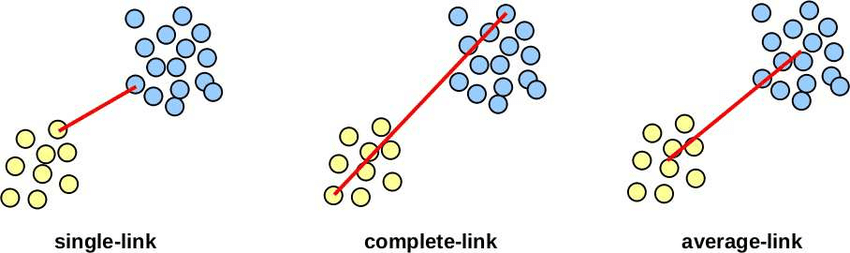
\includegraphics[width=0.8\textwidth]{images/linkage_types}
    \caption{To calculate the distance between two clusters, single linkage calculates the nearest neighbor distance, complete linkage uses the farthest neighbor and average linkage calculates the average distance over all points \cite{linkage_types}.}
    \label{fig:linkage_types}
\end{figure}

\paragraph{Effects of different linkage strategies.}

Depending on the linkage strategy, the pairwise distances between all $N$ clusters $C_1, ..., C_N$ are different for all clusters containing more than one point. As the clustering algorithm merges the closest pair of clusters in each iteration, the merging clusters $C_i$ and $C_j$ with $i, j \in 1,...,N$ might vary as shown in figure \ref{fig:linkage_effects}, where ten clusters $C_0, ..., C_9$ get clustered with bottom-up hierarchical clustering using the Euclidean distance as the pointwise distance $d(x,y)$ to calculate the pairwise distance according to the three mentioned linkage strategies.

\begin{figure}[h]
    \centering
    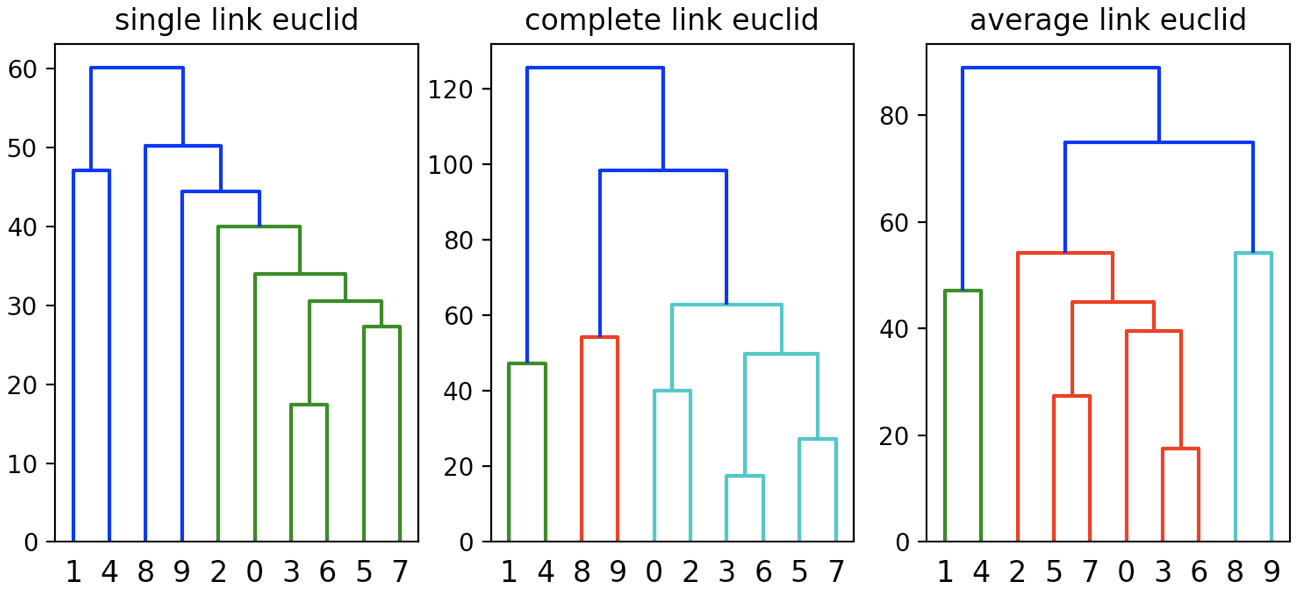
\includegraphics[width=0.8\textwidth]{images/linkage_effects}
    \caption{Different distance measurements often result in different merges for bottom-up hierarchical clustering algorithms. The three discussed linkage strategies result in three different clusterings.}
    \label{fig:linkage_effects}
\end{figure}

As different points are merged together, this also means that the clustering may have a different quality. This thesis compares the clusterings' quality for different data by introducing algorithms to efficiently determine the quality not only for these linkage strategies but also for their linear combinations.

\section{Generating Feature Representations}

In order to improve the overall clustering performance, this work uses several techniques to obtain better feature representations of text and image data. 

\subsection{Text Features}

To cluster different words, there are several ways to create a difference measurement of these words. 

\paragraph{Word Edit Distance.} A rather simple approach would be to calculate the edit distance that describes the difference of the characters in the words \cite{ristad1998learning}. However, this approach does not contain any semantic information, i.e.\ synonyms will have a larger distance than wanted. For example the edit distance between loan and moan (two words with a very different meaning) is very small ($wed(loan, moan) = 1$) where the edit distance between loan and credit (two words with a very similar meaning) is larger ($wed(loan, credit) = 6)$. 

\paragraph{Word Embeddings.} This motivates to leverage contextual information, where we can use several pre-trained models on different datasets. Stanford's GloVe provides such models that incorporate knowledge from Wikipedia and social networks \cite{pennington2014glove}. Figure \ref{fig:glove} shows examples for why these embeddings give a helpful feature representation. 

\begin{figure}[h]
\centering
\begin{minipage}{.3\textwidth}
  \centering
  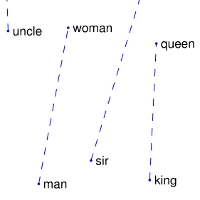
\includegraphics[width=\linewidth]{images/glove_mw}
\end{minipage}
\begin{minipage}{.3\textwidth}
  \centering
  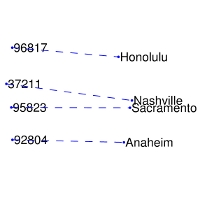
\includegraphics[width=\linewidth]{images/glove_cz}
\end{minipage}
\begin{minipage}{.3\textwidth}
  \centering
  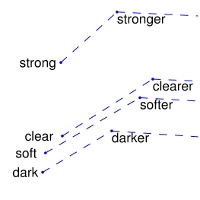
\includegraphics[width=\linewidth]{images/glove_cs}
\end{minipage}
\caption{Word embeddings give insightful correlations between similar and different words. For example, we can obtain several relations between female and male people, between zip codes and cities or between comparative and superlative words \cite{pennington2014glove}.}
\label{fig:glove}
\end{figure}

\paragraph{Bag-of-Contexts.} In addition, CMU's Machine Learning Department provides another way to compare words. Their Never-Ending Language Learner provides information in which contexts certain words are used \cite{nell_pairs}, e.g.\ by considering that both Pittsburgh and Karlsruhe are used in the same context ``\_ is a city'', and Pittsburgh and Philadelphia share additional contexts such as ``\_ belongs to the state Pennsylvania'', we can conclude that Pittsburgh has a higher correlation to Philadelphia than to Karlsruhe. We can then create a corpus containing all different contexts. Similar to the bag-of-words approach \cite{bow}, we then count the occurrences of the words in the corpus' contexts. However, the resulting data is very sparse and the Euclidean distance might not work well to compare the ``bag-of-contexts'' representations, i.e.\ other measurements such as the cosine distance are preferred.

\subsection{Image Features}
\label{sec:imagefeatures}

Similarly, there also exist ways to extract useful features from image data. In particular, this work focuses on neutral networks that learn to represent images in a way that images of different classes can be separated well where images of the same class might share similar features. 

\paragraph{Neural Network Features.} As a primary example, we use Convolutional Neural Network (CNN) architectures that learn to represent images with convolutional, pooling and activation layers and later map the representations to target classes with fully-connected layers. In this way, we can cut off the fully-connected layers to extract lower-dimensional feature representations for the input image data. Figure \ref{fig:cnnfeatures} visualizes such features learned on the ImageNet dataset \cite{krizhevsky2012imagenet}.

\begin{figure}[h]
    \centering
    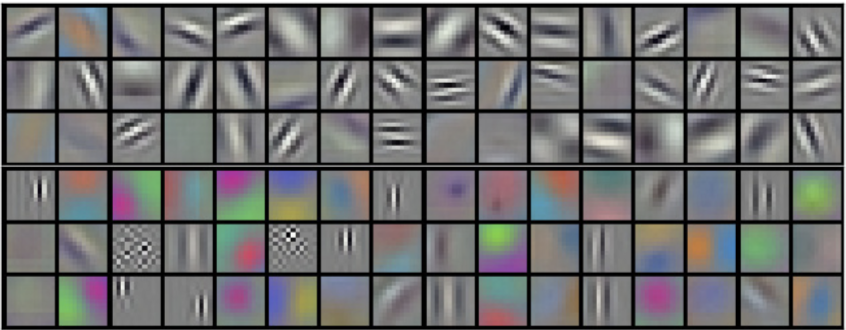
\includegraphics[width=0.7\textwidth]{images/cnn_features}
    \caption{Convolutional Neural Networks learn to represent images in lower-dimensional feature maps by applying convolutions to the image and averaging local neighborhoods (pooling) \cite{krizhevsky2012imagenet}.}
    \label{fig:cnnfeatures}
\end{figure}

\section{Data-Driven Clustering}

As briefly discussed earlier, it is often not trivial to find the best algorithm for a given clustering task. While there already is empirical work in data-driven algorithm selection in certain domains such as choosing the step size in gradient descent \cite{DBLP:journals/corr/GuptaR15b}, this thesis focuses on the earlier discussed bottom-up hierarchical clustering with the three different linkage strategies. In practice, there exists a variety of additional clustering algorithms that often also are parameterized, however data-driven methods only exist to some extent, e.g.\ for calculating the seed points of k-means efficiently \cite{arthur2007k}.\\

As this work tries to select from a family of strategies, we first look at formulations that describe the given families. Balcan et al. introduced two infinite families to interpolate between different linkage strategies, such as shown in equations \ref{eq:algfam1} and \ref{eq:algfam2} \cite{DBLP:journals/corr/BalcanNVW16}.

\begin{equation}
    \begin{aligned}
        \mathcal{A}_1 = \left\{ \left( \min\limits_{u \in A, v \in B} (d(u,v))^\alpha + \max\limits_{u \in A, v \in B} (d(u,v))^\alpha\ \right)^{1 / \alpha} \middle| \alpha \in \mathbb{R} \cup \{\infty, -\infty\} \right\}
    \end{aligned}
    \label{eq:algfam1}
\end{equation}

Equation \ref{eq:algfam1} shows a distance in the range between single linkage ($\alpha = -\infty$) and complete linkage ($\alpha = \infty$). They also show that $\mathbb{R} \cup \{\infty, -\infty\}$ contains a maximum of $O(n^8)$ different intervals, where each interval $[\alpha_{lo}, \alpha_{hi}]$ represents a different merging behavior, i.e.\ a different clustering.

\begin{equation}
    \begin{aligned}
        \mathcal{A}_2 = \left\{ \left( \frac{1}{|A| |B|} \sum\limits_{u \in A, v \in B} (d(u,v))^\alpha \right)^{1 / \alpha} \middle| \alpha \in \mathbb{R} \cup \{\infty, -\infty\} \right\}
    \end{aligned}
    \label{eq:algfam2}
\end{equation}

Equation \ref{eq:algfam2} will also result in single linkage for $\alpha = - \infty$ and complete linkage for $\alpha = \infty$. In addition, the family $\mathcal{A}_2$ also contains the definition of average linkage ($\alpha = 1$). However, the guarantee for maximum $O(n^8)$ intervals does not apply to this family. A formal guarantee will be $O(n^4 2^n)$, but this thesis will show that the empirical results are much better than the actual formal guarantee.\\

Balcan et. al also provide a solution to calculate all different merges of $\mathcal{A}_1$, however this approach solves the mathematical equations and leads to the same clusters being used for a merge quite often. As our solution only evaluates cases where different pairs of clusters get merged, the algorithm described in the following section has a lower runtime as well as a lower complexity.